\setbackground
{
	\centering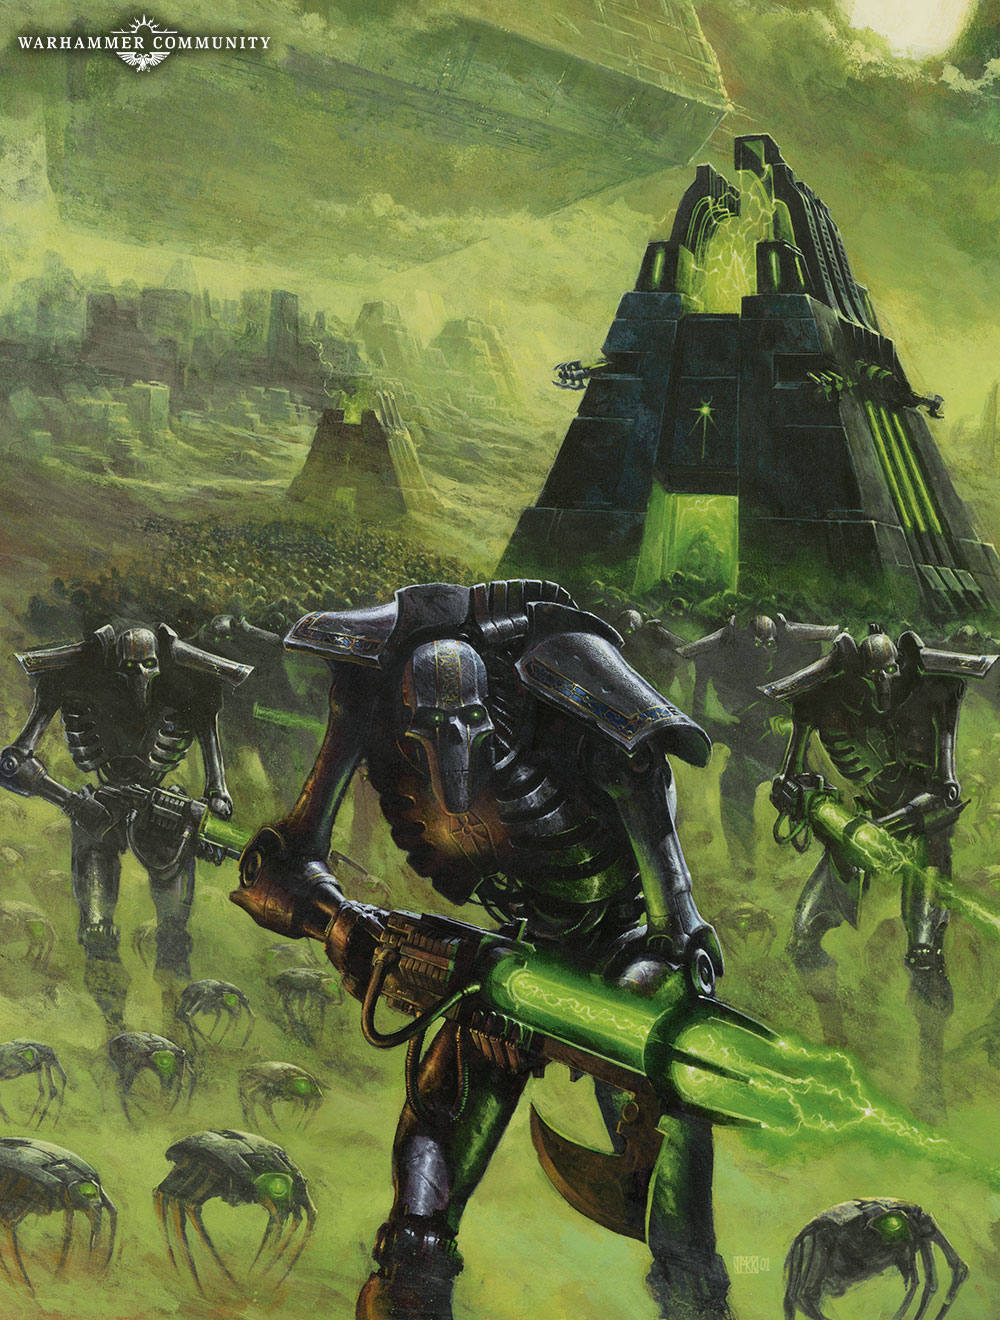
\includegraphics[height=530pt, width=400pt]{troops.jpg}
	\subsection[Troops]{\texorpdfstring{\centering\Huge Troops}{Troops}}
	
	\centerline{\begin{minipage}{400pt}
			\centering
			You have ruled this galaxy for ten thousand of your years, and yet have so little to account to show for your efforts. Such failure must be as depressing to bear as it is shameful to behold!"
			
			\vspace*{1em}
			\raggedleft Imotekh the Stormlord
	\end{minipage}}
}



\newpage
\clearbackground
\subsubsection[Dynastic Warriors Phalanx]{}
\fbox{\begin{imgminipage}{marble.jpg}[t]{0.2\textwidth}
		\color{white}
		\centering {\large TROOPS}
				
		\raggedright \small
		The rank and file of the Necron
		armies are the Dynastic
		Warriors. Silent as the grave,
		Warriors move with slow, erratic,
		yet exacting movements. Despite
		this sluggishness, Warriors are
		capable of great accuracy at
		range and devastating blows up
		close. Like all Necrons, a
		Warrior's living metal
		necrodermis body is incredibly
		durable, capable of absorbing
		truly horrendous amounts of fire
		with hardly a scratch to show for
		it. When enough punishment is
		heaped on a Warrior to actually
		damage it, advanced self-repair
		protocols undo all but the most
		severe damage in moments.
		These seemingly indestructible
		machines carry Gauss Flayers
		which utilise theoretically
		impossible science to strip their
		target apart on a molecular level.
		These potent weapons can strip
		the adamantium from a battle
		tank's hull as surely as they strip
		the flesh from a man. Even
		Power Armour and the enhanced
		constitution of an Astartes
		provide limited defence.
		While the Necron nobility
		retained their personalities and
		intellects intact, their Warriors
		did not come through bio-
		transference so fortunate.
		Warriors possess but a dim
		spark of life, relying in battle on
		orders given through the Nodal
		Command network and
		programmed attack patterns
		rather than any self-direction or
		intellect.
		\color{black}
\end{imgminipage}}
\hspace{0.5em}
\begin{minipage}[t]{0.72\textwidth}
	{\large \textbf{Dynastic Warrior Phalanx \dotfill 60 Points}}
	
	\begin{tabular}{m{165 pt} *{10}{c}}
		 & M & WS & BS & S & T & W & I & A & Ld & Sv \\
		 \hline
		Dynastic Warrior & 5 & 4 & 4 & 4 & 4 & 1 & 2 & 1 & 10 & 4+ \\
	\end{tabular}
	\small
	\begin{minipage}[t]{0.5\textwidth}
		\begin{flushleft}
		\vspace*{2em}
		\textbf{Unit Composition}
		\begin{itemize}
			\item 10 Dynastic Warriors
		\end{itemize}
	
		\textbf{Wargear}
		\begin{itemize}
			\item Bayonet
			\item \quickref{Gauss Flayer}
		\end{itemize}
		\end{flushleft}
	\end{minipage}
	\begin{minipage}[t]{0.5\textwidth}
		\begin{flushleft}
		\vspace*{2em}
		\textbf{Unit Type}
		\begin{itemize}
			\item Infantry (Line, \quickref{Living Metal})
		\end{itemize}
		
		\textbf{Special Rules}
		\begin{itemize}
			\item \quickref{Reanimation Protocols}
			\item \quickref{Soulless Hordes} (Bronze)
			\item Their Number is Legion
			\item Their Name is Death
		\end{itemize}
		\end{flushleft}
	\end{minipage}

	\vspace*{2em}
	\textbf{Weapons}
	
	\begin{tabular}{m{95 pt} *{4}{c} >{\raggedright\arraybackslash}p{130pt}}
		& Range & Type & S & AP & Abilities \\
		\hline
		Bayonet & — & Melee & +1 & — & Two-Handed \\
		\quickref{Gauss Flayer} & 24" & Rapid Fire & 4 & 5 & \quickref{Gauss} (6+)  \\
		\quickref{Gauss Reaper} & 12" & Assault 2 & 5 & 4 & \quickref{Gauss} (6+)  \\
	\end{tabular}

	\vspace*{2em}
	\textbf{Dedicated Transport}
	A Dynastic Warrior Phalanx may take a Night Scythe as a Dedicated Transport, or a Ghost Ark as a Dedicated Transport if it numbers no more than 10 models. As a Dedicated Transport this does not use up an additional Force Organisation slot, but its points cost must still be paid for as part of the army.

	\vspace*{2em}
	\textbf{Options}
	\begin{itemize}
		\item The Dynastic Warrior Phalanx may include:
		\begin{itemize}
			\item Up to an additional 10 Dynastic Warriors \dotfill +7 points each
		\end{itemize}
		\item The entire unit may exchange their \quickref{Gauss Flayer} for a:
		\begin{itemize}
			\item \quickref{Gauss Reaper} \dotfill 0 points each
		\end{itemize}
		\item One Dynastic Warrior may take:
		\begin{itemize}
			\item \quickref{Dynastic Ankh} \dotfill +10 points
		\end{itemize} 
	\end{itemize}
\end{minipage}


\newpage
\subsubsection[Immortals Phalanx]{}
\begin{minipage}[t]{0.72\textwidth}
	{\large \textbf{Immortal Phalanx \dotfill 75 Points}}
	
	\begin{tabular}{m{165 pt} *{10}{c}}
		& M & WS & BS & S & T & W & I & A & Ld & Sv \\
		\hline
		Immortals & 6 & 4 & 4 & 4 & 5 & 1 & 2 & 1 & 10 & 3+ \\
	\end{tabular}
	\small
	\begin{minipage}[t]{0.5\textwidth}
		\begin{flushleft}
		\vspace*{2em}
		\textbf{Unit Composition}
		\begin{itemize}
			\item 5 Immortals
		\end{itemize}
		
		\textbf{Wargear}
		\begin{itemize}
			\item Bayonet
			\item \quickref{Gauss Blaster}
		\end{itemize}
		\end{flushleft}
	\end{minipage}
	\begin{minipage}[t]{0.5\textwidth}
		\begin{flushleft}
		\vspace*{2em}
		\textbf{Unit Type}
		\begin{itemize}
			\item Infantry (Line, \quickref{Living Metal})
		\end{itemize}
		
		\textbf{Special Rules}
		\begin{itemize}
			\item \quickref{Awakening Protocols} (Bronze)
			\item \quickref{Reanimation Protocols}
			\item \quickref{Soulless Hordes} (Silver)
			\item Their Number is Legion
			\item Their Name is Death
		\end{itemize}
		\end{flushleft}
	\end{minipage}
		
	\vspace*{2em}
	\textbf{Weapons}
	
	\begin{tabular}{m{95 pt} *{4}{c} >{\raggedright\arraybackslash}p{130pt}}
		& Range & Type & S & AP & Abilities \\
		\hline
		Bayonet & — & Melee & +1 & — & Two-Handed \\
		\quickref{Gauss Blaster} & 24" & Rapid Fire & 5 & 4 & \quickref{Gauss} (6+)  \\
		\quickref{Tesla Carbine} & 24" & Assault 2 & 5 & — & \quickref{Tesla} (6+)  \\
	\end{tabular}
	
	\vspace*{2em}
	\textbf{Dedicated Transport}
	An Immortal Phalanx may take a Night Scythe as a Dedicated Transport. As a Dedicated Transport this does not use up an additional Force Organisation slot, but its points cost must still be paid for as part of the army.
	
	\vspace*{2em}
	\textbf{Options}
	\begin{itemize}
		\item The Immortal Phalanx may include:
		\begin{itemize}
			\item Up to an additional 5 Immortals \dotfill +15 points each
		\end{itemize}
		\item The entire unit may exchange their \quickref{Gauss Blaster} and Bayonet for a:
		\begin{itemize}
			\item \quickref{Tesla Carbine} and Close Combat Weapon\dotfill -1 points each
		\end{itemize}
		\item One Immortal may take:
		\begin{itemize}
			\item \quickref{Dynastic Ankh} \dotfill +10 points
		\end{itemize} 
	\end{itemize}
\end{minipage}
\hspace{0.5em}
\fbox{\begin{imgminipage}{marble.jpg}[t]{0.2\textwidth}
		\color{white}
		\centering {\large TROOPS}
		
		\raggedleft \small
		As the shock troops of a Tomb
		World's armies, Immortals have
		a far wider range and depth of
		reaction than Warriors, for they
		have retained much of their
		tactical and strategic experience
		from eons ago. Indeed, in many
		ways, the biotransference to
		machine bodies and minds only
		sharpened the Immortals' ability
		to prosecute war in an efficient
		fashion. This is not to say that
		Immortals do not have
		shortcomings. Like all Dynastic
		Legions, they are still inescapably
		tied to the Nodal Command
		matrix and are reliant upon it for
		more advanced order.
		In life, Immortals were the
		professional soldiery of the
		Necrontyr empire. In death, they
		surpass the Warriors in nearly
		every way. Possessed of even
		more resilient frames, Necron
		Immortals prove almost
		impervious to small arms. Their
		training and experience in combat
		survived the process of bio-
		transference undiminished, and
		Immortals seem to have retained
		a brighter spark of intellect than
		their less favoured brethren,
		although only in regard to the
		practice of war. Outside of
		combat, Immortals display about
		as much personality as a
		monotask Servitor. Immortals
		are typically armed with Gauss
		Blasters, weapons even deadlier
		than the Gauss Flayers used by
		Warriors.
		\color{black}
\end{imgminipage}}